\chapter{Design del sistema} % Main chapter title

% \label{Chapter3} % For referencing the chapter elsewhere, use \ref{Chapter2} 
Il primo modello del sistema che si è definito (\textit{modello di analisi}) è stato il risultato della prima fase, ovvero scaturito dalla fase di \textit{analisi e definizione dei requisiti}. \\
\indent L’obiettivo di questo capitolo è invece descrivere il nuovo modello di sistema (\textit{modello di progettazione}), focalizzando l'attenzione prima sull'architettura scelta, poi sulla scomposizione del sistema in sottosistemi e infine sulla descrizione degli obiettivi di design raggiunti.

\section{Modello architetturale client-server}

Lo stile architetturale \textit{client-server} è stato organizzato in tre 
livelli (\textit{tier}) dove ognuno di questi ha un compito preciso e
può essere eseguito su un nodo distinto.

\begin{center}
\renewcommand{\arraystretch}{1.6}
\begin{tabular}{|p{0.25\linewidth}|p{0.25\linewidth}|p{0.42\linewidth}|}
\hline
\textbf{Livello} & \textbf{Realizzazione} & \textbf{Responsabilità} \\
\hline
Presentazione (\textit{client tier}) & Applicazione desktop JavaFX & Mostrare i dati e raccogliere le azioni dell'utente \\
\hline
Logica di business (\textit{application tier}) & Back-end Spring Boot & Validare i dati, applicare le regole di business, autenticare gli utenti e controllarne i permessi \\
\hline
Dati (\textit{database tier}) & Database MySQL & Memorizzare i dati in modo permanente e mantenerli coerenti \\
\hline
\end{tabular}
\end{center}

\subsection{Livello di presentazione (\textit{client-tier})}
Il livello di presentazione costituisce l'interfaccia utente (UI) del sistema e include 
la definizione dei layout visuali, delle schermate e della User Experience 
(UX) complessiva. Per lo sviluppo di questa applicazione desktop si è optato per 
l'impiego della libreria JavaFX.

Questo layer assolve a due funzioni primarie:
\begin{quote}
\begin{enumerate}[label=\textit{\arabic*}]
   \item (\textit{Visualizzazione dei dati}): eroga a schermo le informazioni precedentemente elaborate dal server.
  
  \item (\textit{Acquisizione degli input}): intercetta le interazioni dell'utente (eventi di puntamento, digitazione di testo, selezioni da menu) e le inoltra ai livelli sottostanti. 
\end{enumerate} 
\end{quote}

Il funzionamento si articola su un modello lineare: il livello riceve la richiesta dell'utente, la delega al layer della logica applicativa per la relativa elaborazione e, infine, renderizza il risultato ottenuto. \\
\indent In linea con i principi di separazione delle responsabilità, questo livello non implementa alcuna logica decisionale: non valuta la validità o l'ammissibilità delle operazioni richieste, ma si limita a demandare tali verifiche al livello sottostante e a rappresentare graficamente l'esito della risposta ricevuta.

\subsection{Livello della logica business (\textit{application-tier})}
Il livello della logica applicativa rappresenta il modulo centrale del sistema: in esso risiedono i processi decisionali 
e l'esecuzione delle operazioni fondamentali per il funzionamento dell'applicazione. \\
\indent Per lo sviluppo di questo layer è stato impiegato il linguaggio Java unitamente al framework Spring.
Il layer risponde all'architettura sottostante esponendo le proprie 
funzionalità al livello di presentazione tramite API REST con scambio 
dati in formato JSON. Contestualmente, si interfaccia con il livello 
dei dati (Data Access Layer) per le operazioni di persistenza, lettura 
e aggiornamento delle informazioni.

\subsection{Livello di gestione dei dati (\textit{database-tier})}
Il livello di persistenza è responsabile della memorizzazione a lungo termine, 
del recupero e della salvaguardia della coerenza delle informazioni. \\
\indent La coerenza è garantita
dai vincoli dello schema, come le chiavi esterne, che impediscono per esempio di avere
un’issue senza autore. Al database accede solo il back-end: il client non comunica mai
direttamente con esso.

\subsection{Perché conviene separare i livelli}
I vantaggi di un'architettura a livelli sono:

\begin{quote}
\begin{enumerate}[label=\textit{\arabic*}]
   \item (\textit{Manutenibilità}): Ogni componente ha una singola responsabilità. Trovare e correggere gli errori diventa più rapido e intuitivo.
  
  \item (\textit{Flessibilità}): I moduli sono indipendenti. È possibile rinnovare l'interfaccia (es. da desktop a web) o cambiare il database senza impattare sul resto del sistema.

  \item (\textit{Sicurezza}): Il database rimane isolato dagli accessi esterni diretti, mentre l'autenticazione e il controllo degli accessi sono gestiti in un unico punto sul server. 
  
  \item (\textit{Scalabilità}): I livelli possono essere eseguiti 
  su macchine diverse, come descritto nel paragrafo riguardante il deployment.
\end{enumerate} 
\end{quote}

\section{Decomposizione del sistema}
Il sistema software in esame è stato progettato adottando un approccio modulare, partendo da componenti elementari più facilmente gestibili in fase di sviluppo e manutenzione. \\
\indent In coerenza con l'architettura scelta, il sistema si articola in due macro-sottosistemi: \textit{Front-end} e \textit{Back-end}. Lo sviluppo del primo è stato affidato a Giandomenico Iameo, mentre il secondo a Ubaldo Musto. \\
\indent Ciascun sottosistema è stato a sua volta suddiviso in moduli minori, seguendo il principio di separazione delle responsabilità. \\
\indent Nel seguente paragrafo, verranno descritti dapprima i pattern architetturali utilizzati per la strategia di comunicazione tra i diversi componenti del sottosistema, per poi mostrare la stratificazione del sottosistema stesso.

\subsection{Front-end}
Il \textit{Front-end} provvede alla rappresentazione dei dati e a tutte le interazioni con l'utente. \\
\indent La soluzione adottata per suddividere i moduli presenti all'interno di questo sottosistema si basa sul pattern \textbf{MVP-Passive} \textit{(Model-View-Presenter)}. Per una trattazione approfondita dei meccanismi di funzionamento e delle specifiche di questo pattern, si rimanda all'apposito paragrafo dedicato.

Il diagramma successivo mostra la stratificazione del front-end e la collaborazione tra gli strati stessi.

\begin{figure}[!ht] 
\begin{center}
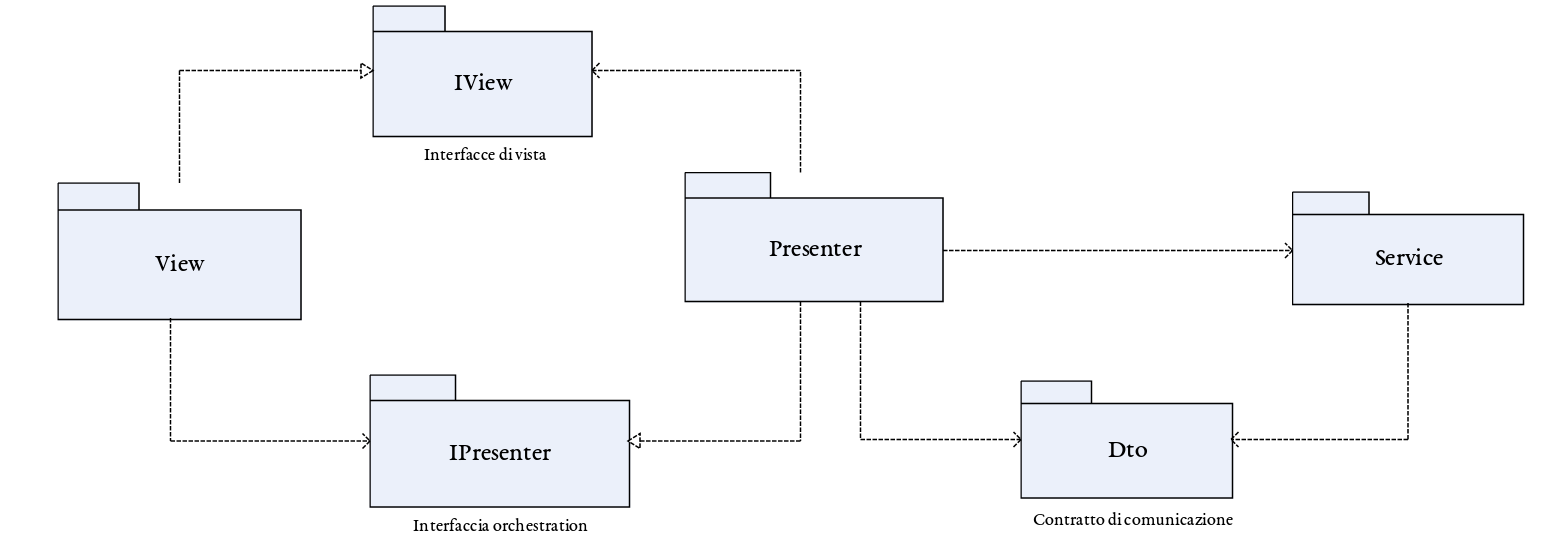
\includegraphics[width=13cm]{Chapters/pattern-front-end.png}
\end{center}
\caption{Diagramma dei package del front-end}
\label{fig:f1} 
\end{figure}

I componenti grafici e il layout dell'applicazione si trovano nello strato \textit{View}. Non contengono logica sui dati, ma si limitano a ricevere i valori già pronti dallo strato \textit{Presenter} e ne invocano i contratti t
ramite le interfacce di \texttt{IPresenter}. \\
\indent Sebbene la logica applicativa sia definita altrove, i componenti grafici mantengono comunque una natura reattiva rispetto alle interazioni dell’utente: a questo scopo, sono state configurate le azioni in risposta agli eventi generati dall'utente. 

Il \textit{Presenter} rappresenta lo strato di orchestrazione. Il funzionamento di questo strato si basa su un modello lineare: Il \textit{Presenter} intercetta i dati provenienti dalle interfacce di vista, converte tali dati in conformità con il contratto di comunicazione definito con il back-end e inoltra la richiesta. Successivamente riceve l'esito della chiamata dal server e, avvalendosi di un componente di mapping (mapper), adatta i dati ricevuti per restituirli alla \textit{View} pronti per la visualizzazione.

Rispetto al classico modello MVP, il front-end non integra un \textit{modello di dominio} locale, ma si affida a uno specifico strato \textit{Service} che comunica direttamente con il \textit{Model} del back-end. Il modello espresso dal front-end è più precisamente un \textit{modello di presentazione}. \\
\indent Più nel dettaglio, a livello di vista è stato adottato il \textit{pattern Composite} per organizzare i componenti grafici in una struttura ad albero. La motivazione che ha spinto a scegliere tale pattern risiede nella natura del toolkit grafico di JavaFX: la cui architettura si fonda nativamente su un grafo di nodi. \\
\indent Il DTO, invece, rappresenta il \textit{modello dei dati} e, insieme all’albero dei componenti grafici, rappresenta l'unico altro modello definito all'interno del sottosistema.

La ragione che ha indotto a non definire un \textit{modello di dominio} locale è di natura progettuale: 
Il front-end è un client "leggero": riceve i dati dal server in formato DTO, li traduce e li mostra. Un livello \textit{domain} avrebbe duplicato quello del server senza aggiungere regole.

% Gli strati di \textit{Adattamento} e \textit{Dati condivisi} non fanno parte di questo flusso, ma sono di supporto allo strato di \textit{Orchestrazione}. Il package \textit{Adattamento} traduce i dati in due sensi: costruisce le richieste da inviare al package \textit{Servizi} e converte le risposte in elementi visualizzabili, tramite interfacce che lo strato di \textit{Presentazione} implementa. Il package \textit{Dati condivisi} definisce il formato delle informazioni scambiate con il back-end ed è usato da  tutti gli strati che le maneggiano. Nessuno dei due è un passaggio obbligato per la richiesta: sono strumenti che l'orchestrazione impiega per trasformare correttamente i dati provenienti dall'interfaccia in richieste accettabili dal backend e le risposte del back-end in elementi che l’interfaccia può mostrare. \\ \\

\subsubsection{Pattern MVP-\textit{Passive}}
MVP-Passive è un modello architetturale comunemente utilizzato nello sviluppo 
di applicazioni mobili e desktop. Si tratta di un'evoluzione del modello MVC (\textit{Model-View-Controller}), incentrato su una separazione delle responsabilità che garantisce maggiore flessibilità e scalabilità.  \\
\indent Il modello MVP è noto principalmente per semplificare la manutenibilità dell'applicazione, favorendone il miglioramento e la scalabilità nel tempo.

Le proprietà principali di questo modello sono la rappresentazione dei dati e la definizione della logica di business dell'applicazione. È responsabile del recupero, dell'archiviazione e della manipolazione dei dati, nonché dell'applicazione delle regole aziendali. Il modello è indipendente dall'interfaccia utente e dovrebbe essere indipendente dall'implementazione specifica della vista (\textit{View}) e del presentatore (\textit{Presenter}).

Il pattern si articola in tre componenti principali, come si nota dalla Figura 1.2.

\begin{figure}[!ht] 
\begin{center}
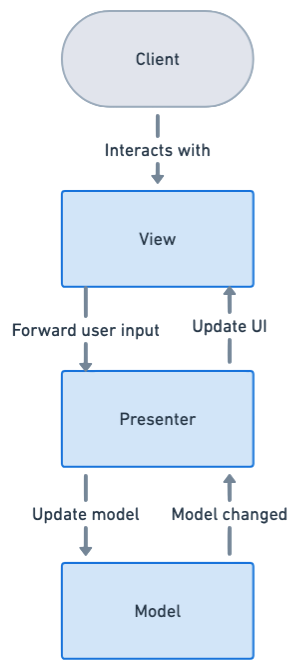
\includegraphics[width=4cm]{Chapters/pattern.png}
\end{center}
\caption{Pattern MVP-passive}
\label{fig:f1} 
\end{figure}

\begin{quote}
\begin{enumerate}[label=\textit{\arabic*}]
   \item (\textit{View}): È responsabile della presentazione dei dati e dell'acquisizione dell'input dell'utente. È un \textit{componente passivo} che si basa sul \textit{Presenter} per aggiornare il proprio stato e gestire le interazioni dell'utente. \\
   La vista in genere è costituita da elementi visivi come i componenti grafici dell'interfaccia utente (UI) e il layout dell'applicazione.
   L'obiettivo principale di View è garantire che l'interfaccia utente sia reattiva, visivamente accattivante e facile da navigare.
  
  \item (\textit{Presenter}): Il \textit{Presenter} funge da mediatore tra \textit{Model} e \textit{View}, orchestrando il flusso di dati e gestendo le interazioni dell'utente. È responsabile del recupero dei dati dal \textit{Model}, della loro elaborazione e dell'aggiornamento della \textit{View} di conseguenza. \\
   Il \textit{Presenter} gestisce inoltre gli eventi utente dalla \textit{View}, come i clic sui pulsanti o le modifiche di input, attivaando azioni specifiche in base a questi eventi. \\
   Separando gli aspetti della gestione dei dati (\textit{Model}), dell'interfaccia utente (\textit{View}) e della componente di presentazione
  (\textit{Presenter}), il pattern consente lo sviluppo di applicazioni più modulari, scalabili e manutenibili.

  \item (\textit{Model}):  rappresenta i dati e la logica aziendale 
  dell'applicazione, simile al modello in MVC. È responsabile dell'
  elaborazione, archiviazione e gestione dei dati e dell'implementazione 
  di tutte le regole aziendali necessarie. Il modello non comunica 
  direttamente con la vista.
\end{enumerate} 
\end{quote}

Concludendo questo paragrafo sugli obiettivi che permette di raggiungere questo pattern, si possono certamente menzionare la separazione delle responsabilità tra i componenti, la manutenibilità e la scalabilità dell'applicazione; proprietà fondamentali che consentono di soddisfare le richieste in continua evoluzione da parte dei clienti. \\
\indent Come esemplificato da molte piattaforme, il modello può essere integrato perfettamente in vari strumenti e metodologie di sviluppo, consolidando ulteriormente la sua rilevanza e importanza nel mondo dello sviluppo di applicazioni. \\

Nel progetto i ruoli del pattern sono realizzati 
come segue. La \emph{View} comprende le schermate e i 
componenti grafici descritti dai file FXML; il \emph{Presenter} 
comprende gli orchestrator e i loro collaboratori (assembler e mapper); 
il \emph{Model} risiede nel back-end, che il front-end raggiunge 
attraverso il livello \texttt{Service} e il package \texttt{dto}. \\
\indent Rispetto alla formulazione classica, il \textit{Presenter} è articolato 
in più componenti ed è associato alle funzionalità anziché alle 
singole schermate; \textit{View} e \textit{Presenter} si conoscono soltanto tramite 
le interfacce dei livelli \textit{IView} e \textit{IPresenter}.

\subsubsection{Stratificazione e partizionamento del sottosistema}
Il sottosistema front-end è stato ulteriormente decomposto in parti più 
piccole in base alle responsabilità che ricopre; come si evince dalla 
Figura 3.5 riportata qui di seguito.

\begin{figure}[!ht] 
\begin{center}
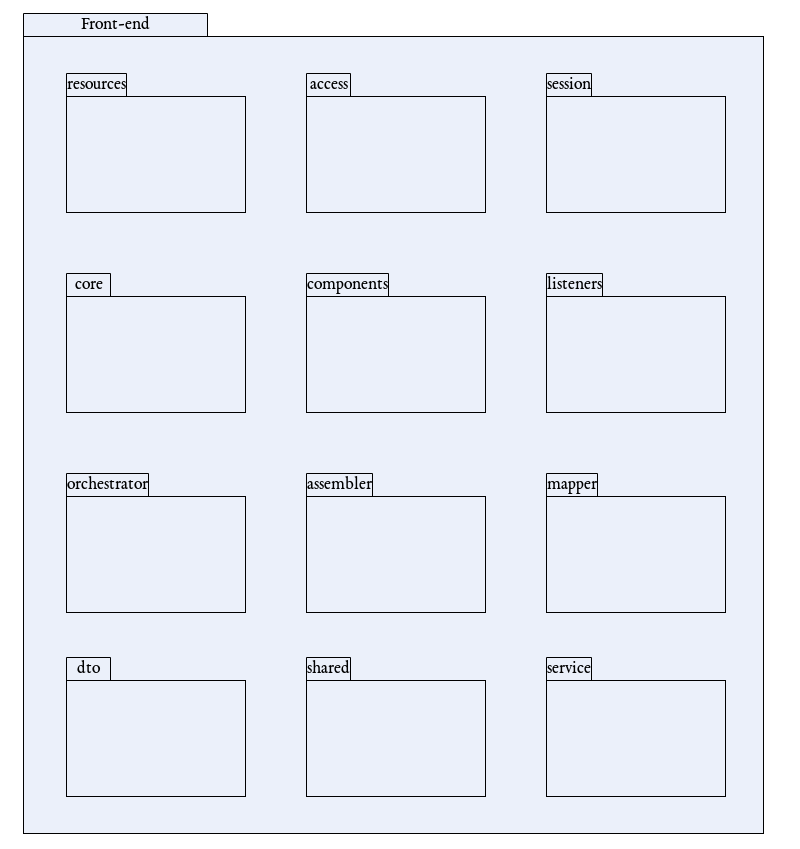
\includegraphics[width=10cm]{Chapters/front-end.png}
\end{center}
\caption{Front-end}
\label{fig:f1} 
\end{figure}

\begin{center}
	\vspace*{-1em}
\def\arraystretch{2.0}
\begin{tabular}{|p{0.17\linewidth}|p{0.18\linewidth}|p{0.55\linewidth}|}
\hline
\textbf{Package} & \textbf{Dimensione} & \textbf{Descrizione} \\
\hline 
\texttt{resources} & Partizione (\textit{View}) & Raccoglie la descrizione dei componenti grafici 
dell'applicazione, definita per mezzo di file FXML. Ogni file è associato 
a un controller, cioè a una classe appartenente allo stesso strato \texttt{View}, 
che ne definisce il comportamento in risposta alle interazioni dell’utente. \\
\hline
\texttt{access, session, components, listeners} & Partizioni (\textit{View}) & Raccolgono le 
classi associate ai componenti grafici dell’interfaccia, cioè i controller 
dei file FXML. Le classi non sono slegate tra loro: si inseriscono nella 
struttura ad albero fornita dal pacchetto \texttt{core}, che riflette 
la composizione gerarchica dei componenti descritti dai file FXML. \\ 
\hline
\texttt{core} & Partizione (\textit{View}) & Data la natura gerarchica 
delle interfacce grafiche, il package \texttt{core} adotta il pattern 
\textit{Composite}: ogni vista è composta da componenti, a loro volta 
composti da altri componenti. Il legame è una composizione ricorsiva. 
Questo ha permesso di semplificare la gestione del ciclo di vita degli 
oggetti: quando una vista viene rimossa, vengono rilasciati anche tutti 
i componenti che la compongono. \\
\hline
\texttt{orchestrator} & Partizione (\textit{Presenter}) & Coordina il percorso dei dati tra 
l’interfaccia grafica e lo strato \textit{Service}, nei due 
sensi. Ogni richiesta originata dall’utente raggiunge questo strato, 
che si avvale dei pacchetti \texttt{assembler} e \texttt{mapper} per costruire una 
richiesta in un formato comprensibile al back-end e la inoltra al 
servizio competente. In modo analogo, ogni risposta ricevuta dal 
back-end viene affidata a questa componente, che la 
converte in elementi visualizzabili dall’interfaccia. \\

\end{tabular} 
\end{center}

\begin{center}
	\vspace*{-2em}
\def\arraystretch{2.0}
\begin{tabular}{|p{0.17\linewidth}|p{0.18\linewidth}|p{0.55\linewidth}|}
\texttt{assembler, mapper} & Partizioni (\textit{Presenter}) & I due pacchetti
traducono i dati nei due sensi. Nel verso dell’invio, \texttt{assembler} converte le 
informazioni provenienti dall’interfaccia in richieste in un formato 
comprensibile al back-end. Nel verso della ricezione, \texttt{mapper} converte le risposte 
del back-end in elementi visualizzabili dall’interfaccia. I pacchetti
non dipendono dai componenti grafici concreti: operano su interfacce che lo 
strato di \textit{View} implementa, così la logica di traduzione 
resta indipendente dalla grafica.\\
\hline
\texttt{dto} & Strato (\textit{Dto}) & Lo strato \texttt{Dto} definisce il contratto di comunicazione con il back-end. Raccoglie le classi DTO, usate come formato standard di scambio delle informazioni. \\
\hline
\texttt{shared} & Trasversale & 
Raccoglie le classi di utilità in comune a più componenti. \\
\hline
\texttt{service} & Strato (\textit{Service}) & Lo strato \textit{Service} gestisce la comunicazione con il back-end: effettua le richieste HTTP e riceve le relative risposte. È l’unico strato a conoscere il protocollo di trasporto, e questo isola il resto del sottosistema dai dettagli della comunicazione. Le richieste e le risposte sono rappresentate da oggetti DTO, che i servizi ricevono dallo strato di \textit{Presenter} e a cui restituiscono i risultati. \\
\hline
\end{tabular} 
\end{center} 

\vspace{1cm}

\subsection{Back-end: pattern Controller-Service-Repository}
Il back-end è organizzato in livelli secondo il pattern Controller-Service-Repository. 
Lo abbiamo scelto perché 
separa in modo netto le responsabilità: i controller gestiscono la comunicazione 
HTTP con il client, i service contengono tutte le regole di business e i 
repository l'accesso al database. \\
\indent In questo modo la logica si trova in un 
unico punto e può essere riusata da più endpoint, ogni livello può cambiare 
senza toccare gli altri e i service possono essere testati in isolamento, 
sostituendo i repository con dei mock.

\begin{figure}[!ht]
\begin{center}
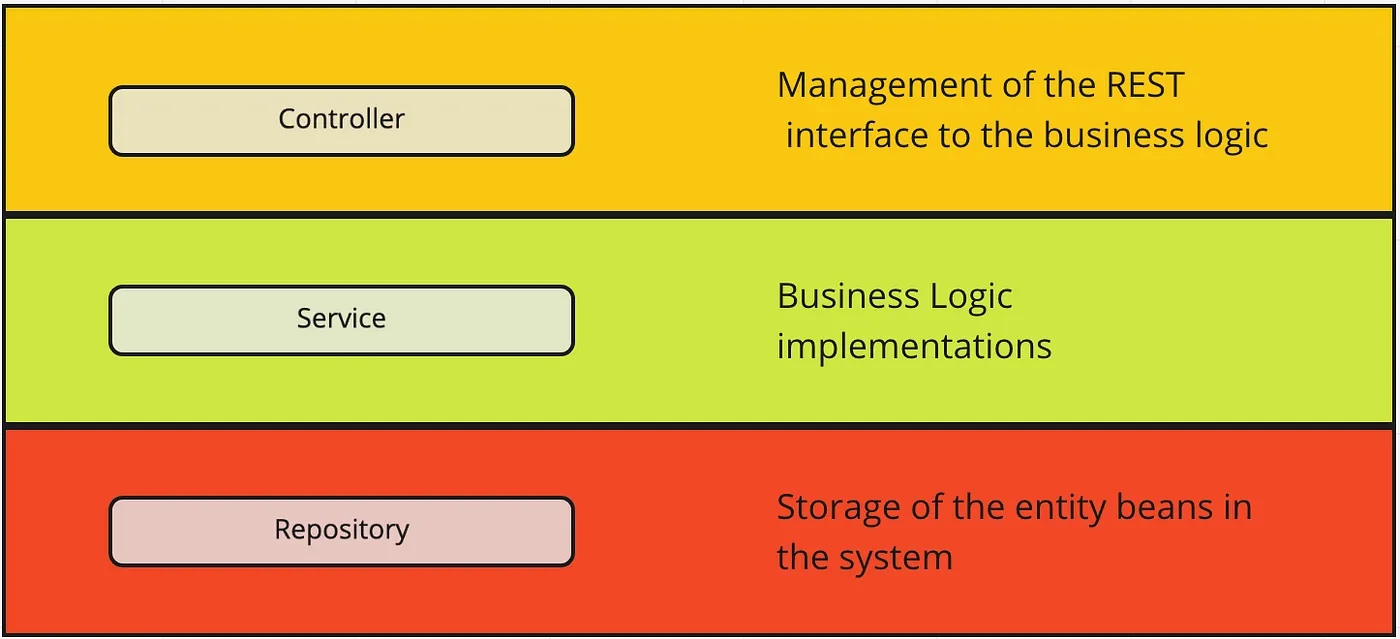
\includegraphics[width=10cm]{Chapters/controller.jpeg}
\end{center}
\caption{Pattern Controller-Service-Repository}
\label{fig:controller-service-repository}
\end{figure}

\begin{itemize}
  \item \textit{Controller}: In cima allo schema, ha il solo compito di esporre le funzionalità del sistema come API REST, in modo che possano essere usate da entità esterne, come il client.
  \item \textit{Service}: Contiene tutta la logica di business. Se ha bisogno di leggere o salvare dati, si rivolge a un repository; chi vuole accedere alla logica di business deve passare da un controller.
  \item \textit{Repository}: In fondo allo schema, ha il compito di salvare e recuperare un certo insieme di dati.
\end{itemize}

\subsection{Back-end: Repository pattern}
Per l'accesso ai dati abbiamo adottato il Repository pattern, che offre ai service un modo astratto di lavorare con i dati. Ogni entità del dominio ha un proprio repository, che si comporta come una collezione di oggetti: i service possono cercare, salvare ed eliminare elementi senza sapere come sono memorizzati nel database. \\
\indent I repository sono interfacce: le operazioni CRUD di base (creazione, lettura, aggiornamento ed eliminazione) sono ereditate da Spring Data JPA, che ne genera l'implementazione, mentre le ricerche con filtri e ordinamenti sono query aggiuntive dichiarate nell'interfaccia stessa. In questo modo i service non contengono query né dettagli delle tabelle: un cambiamento nello schema si riflette sui repository e non sui service.

\begin{figure}[!ht]
\begin{center}
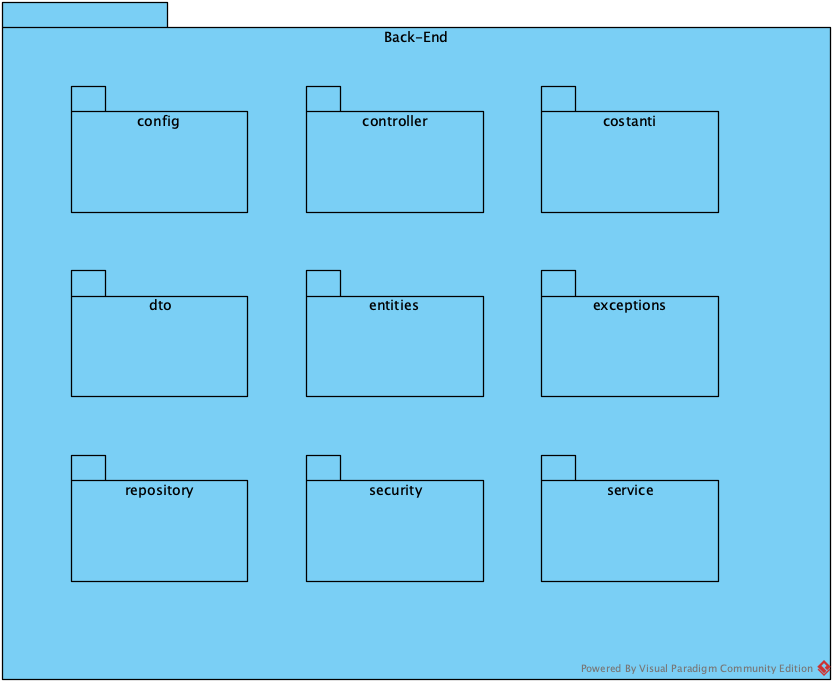
\includegraphics[width=8cm]{Chapters/Immagine.png}
\end{center}
\caption{Decomposizione del back-end}
\label{fig:decomposizione-back-end}
\end{figure}


%----------------------------------------------------------------------------------------
\section{Comunicazione tra front-end e back-end}
Il client e il server comunicano tramite API REST su HTTP. Ogni operazione dell'utente corrisponde a una richiesta HTTP, con dati in formato JSON sia in richiesta sia in risposta; fanno eccezione le immagini allegate alle issue, che vengono scaricate con una richiesta separata come dati binari, per non appesantire gli elenchi. \\
\indent Gli errori hanno sempre lo stesso formato: un codice HTTP (per esempio 400 per dati non validi, 403 per permessi insufficienti, 404 per una risorsa inesistente) e un corpo JSON con un messaggio che il client può mostrare all'utente.

\subsection{Autenticazione}
L'autenticazione usa Spring Security con la sessione HTTP: al login il server verifica email e password, crea una sessione e restituisce al client un cookie, che il client allega a tutte le richieste successive. Le password sono salvate solo come hash BCrypt. \\

\subsection{Interfaccia delle API}
La tabella seguente riassume gli endpoint esposti dal back-end. Tutti, tranne il login, richiedono l'autenticazione.

\begin{center}
\renewcommand{\arraystretch}{1.4}
\begin{tabular}{|p{0.10\linewidth}|p{0.38\linewidth}|p{0.18\linewidth}|p{0.24\linewidth}|}
\hline
\textbf{Metodo} & \textbf{Endpoint} & \textbf{Ruolo} & \textbf{Funzionalità} \\
\hline
POST & \texttt{/api/auth/login} & pubblico & Login \\
GET & \texttt{/api/auth/me} & autenticato & Utente collegato \\
POST & \texttt{/api/auth/logout} & autenticato & Logout \\
\hline
POST & \texttt{/api/utenti} & amministratore & Crea utente \\
GET & \texttt{/api/utenti} & amministratore & Elenco utenti \\
GET & \texttt{/api/utenti/suggeriti} & amministratore & Suggerimento assegnatari \\
\hline
GET & \texttt{/api/issues} & autenticato & Elenco con filtri e ordinamento \\
GET & \texttt{/api/issues/ricerca} & autenticato & Ricerca per parola chiave \\
GET & \texttt{/api/issues/\{id\}} & autenticato & Dettaglio issue \\
GET & \texttt{/api/issues/\{id\}/immagine} & autenticato & Immagine allegata \\
POST & \texttt{/api/issues} & amm., normale & Crea issue \\
POST & \texttt{/api/issues/\{id\}/chiudi} & amministratore & Chiudi issue \\
\hline
POST & \texttt{/api/bugs/\{id\}/assegna} & amministratore & Assegna bug \\
POST & \texttt{/api/bugs/\{id\}/duplicato} & amministratore & Segna come duplicato \\
GET & \texttt{/api/bugs/assegnati} & normale & Bug assegnati \\
GET & \texttt{/api/bugs/assegnati/aperti} & normale & Bug assegnati aperti \\
\end{tabular}
\end{center}

\begin{center}
\renewcommand{\arraystretch}{1.4}
\begin{tabular}{|p{0.10\linewidth}|p{0.38\linewidth}|p{0.18\linewidth}|p{0.24\linewidth}|}
GET & \texttt{/api/notifiche} & normale & Tutte le notifiche \\
GET & \texttt{/api/notifiche/conteggio} & normale & Numero di notifiche nuove \\
POST & \texttt{/api/notifiche/leggi-nuove} & normale & Legge le notifiche nuove \\
\hline
\end{tabular}
\end{center}
%----------------------------------------------------------------------------------------

\vspace{1cm}

\section{Deployment}
Il diagramma di deployment mostra come i componenti software sono distribuiti sui nodi di esecuzione.

\begin{figure}[!ht]
\begin{center}
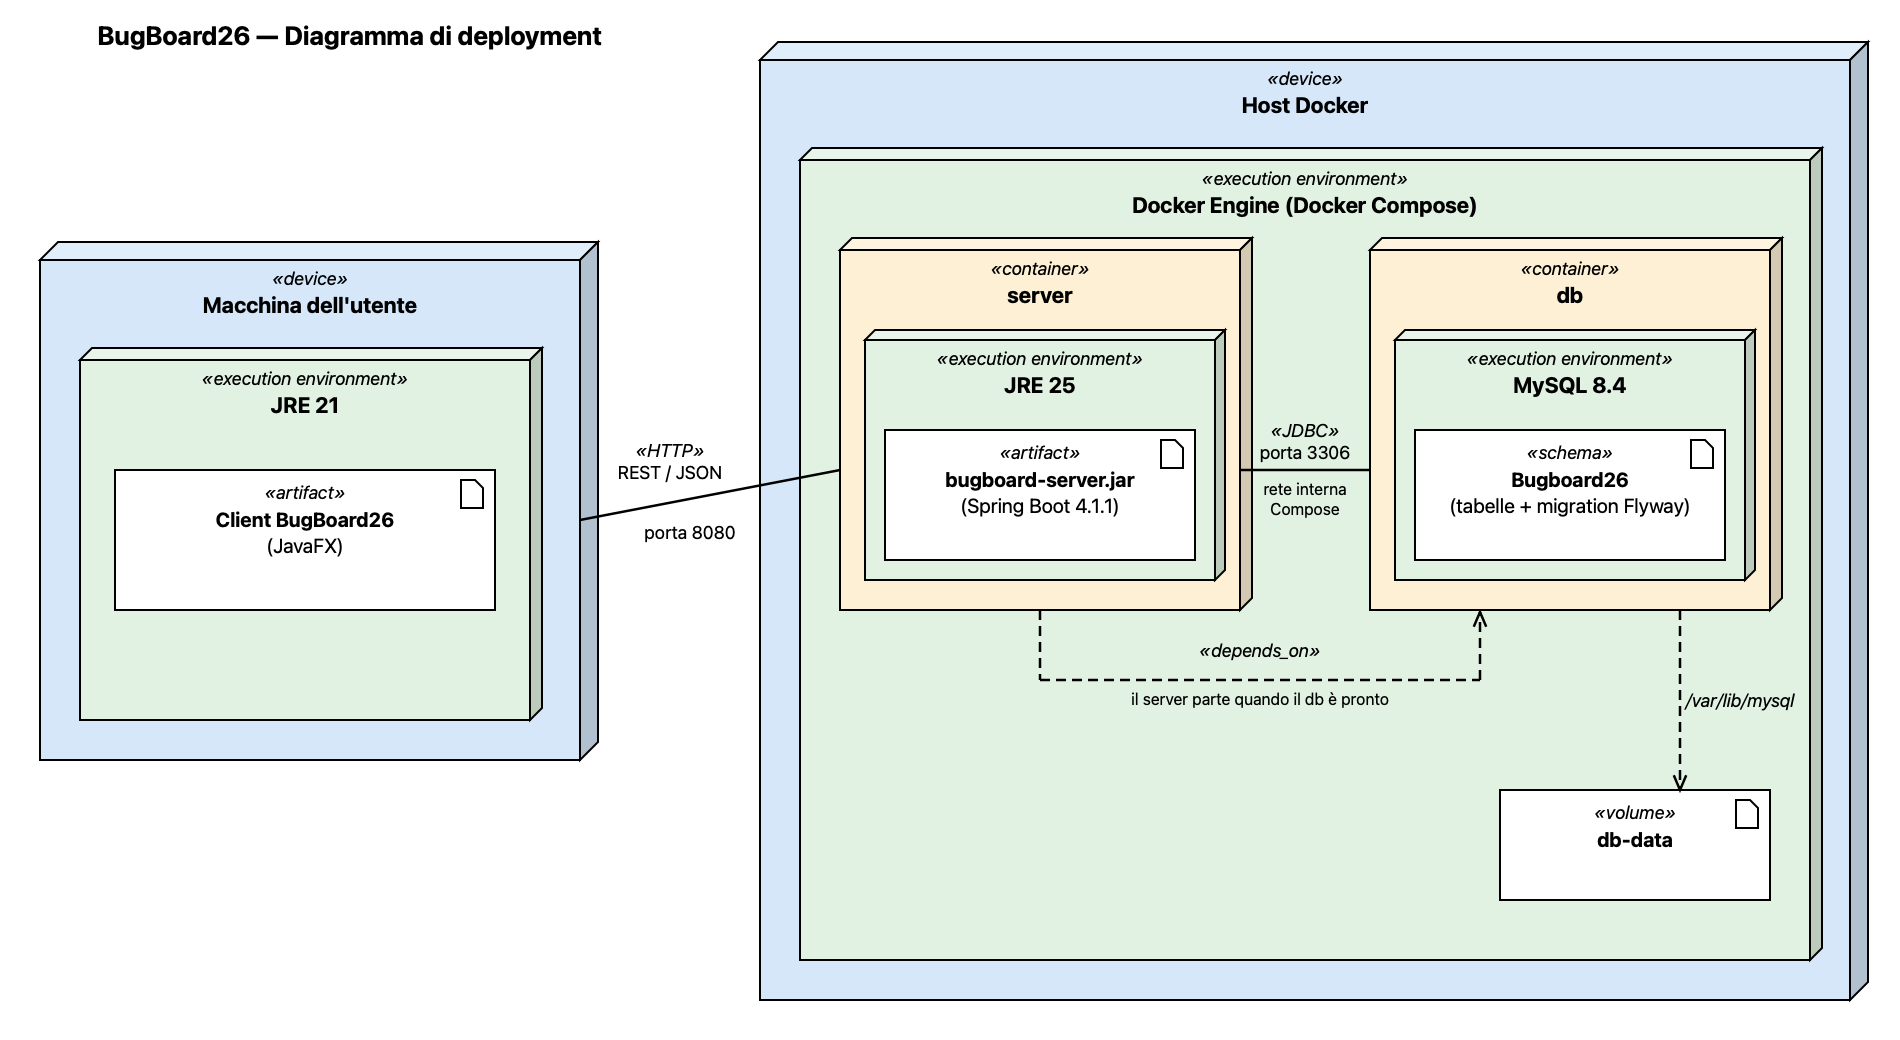
\includegraphics[width=\linewidth]{Chapters/image.png}
\end{center}
\caption{Diagramma di deployment}
\label{fig:deployment}
\end{figure}

\begin{itemize}
  \item \textit{Macchina dell'utente}: esegue il client JavaFX, che richiede un ambiente Java 21.
  \item \textit{Host Docker}: esegue due container avviati insieme da Docker Compose. Il container \textit{server} contiene il back-end Spring Boot con il runtime Java 25 ed è raggiungibile sulla porta 8080; il container \textit{db} contiene MySQL 8.4 e salva i dati in un volume, così non si perdono quando il container viene ricreato.
  \item \textit{Comunicazioni}: il client comunica con il back-end tramite HTTP, scambiando dati in formato JSON; il back-end comunica con il database tramite JDBC, sulla rete interna creata da Docker Compose.
\end{itemize}

Client e back-end si trovano quindi sempre su nodi distinti. Back-end e database sono in container separati e, nella configurazione consegnata, sullo stesso host; per spostarli su macchine diverse basta cambiare l'indirizzo del database nella configurazione del back-end.
%----------------------------------------------------------------------------------------
\section{Criteri di design}
\begin{itemize}
  \item \textit{Separazione delle responsabilità}: ogni livello e ogni componente ha un solo compito. Il principio è applicato a tutti i livelli: nell'architettura a tre livelli, nel pattern Controller-Service-Repository del back-end e nel pattern MVP del front-end.
  \item \textit{Indipendenza tra front-end e back-end}: le due parti comunicano solo tramite API REST, secondo un contratto definito dai DTO. Il back-end non conosce il client, che può essere sostituito senza modifiche al server.
  \item \textit{Stato e regole centralizzati}: dati, regole di business e controlli dei permessi stanno solo nel back-end. Il client mostra i dati e inoltra le richieste, ma non prende decisioni.
  \item \textit{Astrazione per il riuso e l'estensione}: i ruoli degli utenti e i tipi di issue sono gerarchie di classi, l'accesso ai dati passa per interfacce \textit{repository} e i componenti grafici seguono il pattern \textit{Composite}.
  \item \textit{Sicurezza per default}: ogni operazione, tranne il login, richiede l'autenticazione, e i permessi sono dichiarati su ogni endpoint.
  \item \textit{Testabilità}: i service dipendono dai repository solo tramite interfacce, quindi possono essere testati in isolamento sostituendo i repository con dei mock.
\end{itemize}

%----------------------------------------------------------------------------------------

\section{Scelte tecnologiche}

\begin{center}
\renewcommand{\arraystretch}{1.4}
\begin{tabular}{|p{0.3\linewidth}|p{0.6\linewidth}|}
\hline
\textbf{Ambito} & \textbf{Tecnologia} \\
\hline
Front-end & Java, JavaFX \\
Back-end & Java, Spring Boot (Web, Data JPA, Security, Validation) \\
Database & MySQL \\
Gestione dello schema & Flyway \\
Distribuzione & Docker, Docker Compose \\
\hline
\end{tabular}
\end{center}

\subsection{Spring Boot}
Per il back-end abbiamo scelto Spring Boot, il framework più diffuso per lo sviluppo di servizi REST in Java. Spring Boot segue il paradigma \textit{convention over configuration}: fornisce una configurazione predefinita ragionevole per gli aspetti più comuni (server web integrato, connessione al database, conversione JSON), così gli sviluppatori devono specificare solo ciò che si discosta dallo standard. Questo riduce il codice di configurazione e il numero di decisioni da prendere, senza perdere flessibilità: ogni impostazione predefinita può essere sovrascritta quando serve. \\
\indent Spring offre inoltre la \textit{dependency injection}: controller, service e repository vengono creati dal framework e collegati tra loro automaticamente, il che rende i componenti indipendenti e facili da testare. Infine il suo ecosistema mette a disposizione moduli già integrati per tutte le esigenze del progetto: Spring Web per le API REST, Spring Data JPA per l'accesso al database, Spring Security per l'autenticazione e i permessi, Jakarta Validation per il controllo dei dati in ingresso. Usare soluzioni standard e collaudate, invece di scriverle da zero, ci ha permesso di concentrarci sulla logica di business, riducendo gli errori soprattutto in un ambito delicato come la sicurezza.

\subsection{MySQL e Flyway}
Per la persistenza abbiamo usato MySQL, un database relazionale. I dati di BugBoard26 sono strutturati e collegati tra loro (un'issue ha un autore, un bug ha un assegnatario, una notifica ha un destinatario), quindi il modello relazionale, con le sue chiavi esterne e le transazioni, è il più adatto. \\
\indent Lo schema non viene generato dal codice, ma è creato e aggiornato da Flyway tramite script SQL numerati (\textit{migration}), applicati automaticamente all'avvio del back-end. In questo modo ogni installazione, dal computer di sviluppo al container, ha esattamente lo stesso schema.

\subsection{Docker}
Docker è usato per automatizzare la distribuzione del back-end sotto forma di container, cioè un pacchetto che contiene l'applicazione insieme a tutto ciò che le serve per funzionare (il runtime Java e le librerie). Il container si comporta allo stesso modo su qualsiasi macchina, dal computer di sviluppo a un server nel cloud, ed elimina i problemi di installazione e configurazione dell'ambiente. \\
\indent Il Dockerfile è di tipo \textit{multi-stage}: l'applicazione viene compilata in un'immagine con il JDK e Maven, mentre l'immagine finale contiene solo il runtime Java e l'applicazione, quindi è più leggera e non include strumenti di compilazione. Infine, con Docker Compose il back-end e il database MySQL si avviano insieme con un unico comando: il back-end parte solo quando il database è pronto, e i dati vengono conservati in un volume, così non si perdono quando i container vengono riavviati.

\subsection{JavaFX}
Per questa applicazione desktop è stato utilizzato JavaFX come toolkit grafico. Tra i suoi vantaggi merita di essere menzionata la gestione del layout, che permette di separarlo dal codice. Il layout si trova in file FXML, che descrivono in modo dichiarativo i componenti grafici dell’applicazione. Ogni file è associato a un controller, cioè a una classe che ne definisce il comportamento in risposta alle interazioni dell’utente: senza controller l’interfaccia è priva di comportamento. \\\
\indent L’aspetto grafico è definito in fogli di stile CSS e si applica ai componenti tramite classi di stile, senza modificare il codice. Infine, lo stesso codice Java può essere eseguito su più piattaforme, come Windows, macOS e Linux.

\subsection{Linguaggi e strumenti}
Il sistema è stato sviluppato con un linguaggio orientato agli oggetti, Java, usato sia per il back-end sia per il front-end. Usare lo stesso linguaggio nei due componenti ha semplificato lo sviluppo e la collaborazione tra i membri del gruppo.
\begin{itemize}
  \item \textit{Java}: versione 25 per il back-end, con il framework Spring Boot, e versione 21 per il front-end, con la libreria JavaFX.
  \item \textit{SQL}: usato per definire lo schema del database e i dati iniziali, negli script di migrazione gestiti da Flyway.
  \item \textit{JPQL} (\textit{Java Persistence Query Language}): linguaggio di interrogazione simile a SQL, che lavora sulle classi Java invece che sulle tabelle. È usato nei repository per le ricerche con filtri e ordinamenti.
  \item \textit{YAML}: formato del file di configurazione del back-end e del file di Docker Compose.
\end{itemize}
Gli strumenti utilizzati sono:
\begin{itemize}
  \item \textit{IntelliJ IDEA}: ambiente di sviluppo per entrambi i sottosistemi;
  \item \textit{Maven}: gestione delle dipendenze e build automatica del back-end;
  \item \textit{Visual Paradigm} e \textit{Modelio}: strumenti CASE per i diagrammi UML, rispettivamente del back-end e dei casi d'uso, e del front-end;
  \item \textit{MySQL Workbench}: progettazione del modello ER e generazione automatica dello script SQL di creazione delle tabelle;
  \item \textit{Git} e \textit{GitHub}: controllo di versione e hosting dei repository del front-end e del back-end;
  \item \textit{SonarQube}: analisi statica della qualità del codice del back-end.
\end{itemize}